\documentclass[10pt,a4paper,twocolumn]{article}
\usepackage[utf8]{inputenc}

% For dummy texts, can be deleted when we don't use those any more
\usepackage[english]{babel}
\usepackage{blindtext}

% Math packages
\usepackage{amsmath}
\usepackage{amsfonts}
\usepackage{amssymb}
\usepackage{makeidx}

% Various settings
\usepackage{graphicx}
\usepackage[left=2cm,right=2cm,top=2cm,bottom=2cm]{geometry}
\usepackage{tikz}
\usepackage{pgfplots}

\usetikzlibrary{patterns}

% For the \maketilte command
\author{Daniel Damgaard \\
201303575 \\
daniel@damgaard.in
\and
Rohde Fischer \\
20052356 \\
rohdef@rohdef.dk
}
\title{Efficient Position Updating - Team: EagleEye}

\begin{document}
\maketitle

\tableofcontents

\section{Introduction}
\blindtext

\section{Implementation}
The project consists of the following two parts, A) an Android application (Client) and B) a Java application (Server). The client sends locations to the server, which stores the received locations. The client gets the locations of latitude and longitude from the build-in GPS. The client offers some different algorithms for requesting and selecting GPS locations. It makes it possible for the server to track to client.

\subsection{Design choices}
\subsubsection{Algorithms}
The following algorithms is implemented and evaluated.

Periodic Reporting Strategy (PRS): For each specified number of seconds a GPS fix is requested. Each GPS fix is sent to the server.

Distance-based Reporting Strategy (DBRS): The client continuously receive GPS fixes, but only sends the location to the server, when the distance to the last location crosses a specified distance threshold.

Distance-based Reporting Strategy - Accelerometer (DBRS - A): This is an extension of DBRS, where the client only receives GPS fixes when the target is moving according to the accelerometer. If the accelerometer shows no movement, it is assumed that the target is at the last location.

Distance-based Reporting Strategy - Max Speed (DBRS - MS): This is also an extension of DBRS, this time where GPS fixes is requested, when the target is expected to reach the distance threshold when it is moving with a specified max speed. If a GPS fix is requested, but the target has not reached the distance threshold as expected, the GPS fix is discarded and the client waits for the remaining distance to be done.
\subsubsection{Choices at the client}
In two of the algorithms a timer was used to limit the amount of readings from the GPS for the experiments. Due to some permission problems on the platform this is done by sleeping the thread in stead of using the timer. When doing delays based on an assumed maximum speed the delay for the next reading is done as a part of handling the response, to ensure that the delay calculation is done on the newest reading.

For the accelerometer a delay was introduced in the readings to make live analysis of data easier. The analysis was used to find an assumption of when the acceleration was big enough to assume movement. A value of $2 m/s^2$ was found as a reasonable threshold, by simulating walking with the phone and reading the accelerations. The delay was kept in the client during testing to avoid changing the results from our simulations.
\subsubsection{Server protocol - TCP}
\input{chapterExample}
\subsection{User guide}
\blindtext

\section{Evaluation}
To evaluate the project a route around Storcenter Nord with some fix points is chosen. It takes approximately 9 minutes to walk the route, which fits well when two stops of each 1 minute are added. The fix points are the same location across the different algorithms, but with a unique elapsed time measured for each.

\subsection{Periodic Reporting Strategy}
This strategy is measured with the time period set to 1 second, which means we assume roughly 11 * 60 = 660 locations to be sent to the server for the walk. Thus only the place mark correspond to the time of the fix points is shown at the screen shot. 

The first location is placed in the middle of the crossroad, which is probably explained by cold start of the GPS. After that the accuracy fits the fix points B and C quite good. But at point L236 near D where we stopped for 1 minute, there are some fluctuations. Afterwards at point L347 near E the estimated position is placed almost inside the building, which also is a bit off. At point L399 - L457 there is almost no fluctuations, which differs from the last stop. Later at point L523 near H the GPS estimate the position to be at the opposite side of the road. But the last position L615 near I ends to be close to the real position.

The first stop has some fluctuations, while the second stop does not. The GPS is continuously running and therefore high accuracy and no fluctuations is expected at the stops.

Due to the many locations sent to the server, this algorithm does not match the goal of this project, to make efficient position updating with few GPS fixes and few transmissions to achieve low battery consumption.
\subsection{Distance-based Reporting Strategy}
The distance of 50 meters is used for the measurements of this algorithm.

The first location L0 is far off from the real starting point, which assumes to be due to the cold start of the in-build GPS. Afterwards the points L1 - L5 is almost equal to the truth ground. But at the corner C between L5 and L6 the algorithm estimate a straight line, which cut off the real corner. The pause of 1 minute does not effect the path from L6 to L7, which fits well. But point L8 is placed almost inside the building, which makes the corner of L7 - L9 looks like L5 - L6. But it is a different situation because the corner of L7 - L9 should have the point L8 to make the corner right. But due to inaccuracy at point L8, it cut of the corner and make it look like L8 was not there. There is a low accuray at the point L10, which is far of in the building. The reason is not a cold start due of the pause, because the GPS will not turn off due to the regular GPS fixes. The corner of L11 and L12 near G is cut of like the corner at C. The points L13 and L14 fit well to the truth ground.

This algorithm suites best for a static or regular direction, because it has a tendency to cut of corners. It seems like it fits well for the goal of efficient position updating due the few locations, but it uses a lot of GPS fixes to determine when the configured distance is done.
\subsection{Distance-based Reporting Strategy - Max Speed}
During the analysis of the data from the distance based reporting with a maximum speed (MS), the accuracy distances was very high. The accuracy show how precise the location is where a low number indicates that you are close to your target. The DBMS and accelerometer is compared in figure-\ref{maxspeedaccelerometeraccuracy} it can be seen that the accuracies are way worse than for the accelerometer, this can also be seen on the Google Earth plot of the route.

\begin{figure}[h]
\begin{tikzpicture}

\begin{axis}[
width=7cm,
height=6cm,
axis x line*=bottom,
legend style={at={(0.5,1.2)},
anchor=north,legend columns=-1},
xlabel={Location number},
axis y line*=left,
ylabel={Accuracy (m)},
grid=none
]

\addplot[color=blue,mark=none] table {tabledata/DBRSAccelerometer.accuracies};
\addplot[color=red,mark=none] table {tabledata/DBRSMaxSpeed.accuracies};

\legend{Accelerometer, Max speed}
\end{axis}

\end{tikzpicture}

\caption{Comparison of accuracies for the max speed and accelerometer algorithms. Accuracy is how far from our actual location we could be. Measurement number is the index for the reading on the server.}
\label{maxspeedaccelerometeraccuracy}
\end{figure}

The high numbers on the accuracy curve is probably due to the GPS switching off and having to do a cold start[REFERENCES]. This is also suggested by figure-\ref{locationsreadandsent} that shows way fewer readings by MS. The MS algorithm performs very well on the amount of locations read from the GPS at a rate of only $5.4$ messages per minute, but the accuracy should probably be better. It sends fixes to the server at a rate of $1.5$ per minute.
\subsection{Distance-based Reporting Strategy - Accelerometer}
The readings from the accelerometer in figure-\ref{maxspeedaccelerometeraccuracy} have a spike at around location number 8, this indicates a GPS warm up, where the first location have a bad accuracy. From the fact that we had to breaks at one minute each two spikes is actually expected. This could be due to background applications doing GPS readings outside our control. But this can also be due to the accelerometer algorithm being too sensitive, which was also indicated by one of the test runs.

Apart from that the accelerometer seems to have a quite good accuracy of $\leq 6m$, and sends data at a rate of $1.3$ fixes per minute. The accelerometer reads GPS fixes at a rate of $42$ per minute. 
\subsection{Discussion}
% Mandatory: Create screenshots using Google Earth for each of the scenarios of the collected KML files. The screenshots should include a path that marks the actually walked route. Comment on the results in the report and discuss how GPS errors impacted the results.
% Mandatory: Make a list with the following entries for each scenario: strategy, number of GPS fixes, number of uplink messages, time span, GPS fixes per second, uplink messages per second and comment on them in the report with respect to relevant literature. Discuss what pervasive positioning applications the different strategies are relevant for.
\blindtext

\begin{tabular}{l r r r r r}
& Number of & Number of & Time span & GPS fixes & Uplink messages \\
& GPS fixes & uplink messages & in seconds & per second & per second \\
\hline
Periodic Reporting Strategy & 5 & 5 & 44 & 3 & 3 \\
\hline
Distance-based Reporting Strategy & 5 & 5 & 44 & 3 & 3 \\
\hline
DBRS: Accelerometer & 5 & 5 & 44 & 3 & 3 \\
\hline
DBRS: Max Speed & 5 & 5 & 44 & 3 & 3 \\
\hline
\end{tabular}

\section{Reflection}

\subsection{Accuracy}
When the GPS starts from a cold start the uncertainty of the GPS readings is relatively high. In a lot of cases a higher accuracy would be needed, and in these cases it should take multiple readings till some desired accuracy is reached. This could have the downside that it could keep requesting locations when the GPS conditions is bad. Depending on the use case such an algorithm could be designed with a threshold for how many tries to get and then either use the accelerometer to detect movement (the GPS signal conditions should change in this case) or wait for some time before trying again, to save power.
\subsection{Accelerometer}
The accelerometer measurements has the potential for a few improvements. First off our data could suggest that the detection of movement could be improved, a sliding window algorithm would probably improve the accuracy of the movement detection. Basically have the $n$ last magnitude ($\sqrt(x^2+y^2+z^2)-gravity$) readings and take the average of them. This could help remove noise from the user taking the phone or normal phone operations.

Also the threshold used to detect when something is considered as movement should be found by gathering empirical data of peoples movements, to find an appropriate $n$ for the sliding window and a threshold for how much movement that is needed to consider it movement.
\subsection{Uneven movement}
The DBRS algorithms assumes, that the target moves like straight paths and does not change direction to go backwards. The bad scenarios is sketched in figure-\ref{unevenmovement}.

\begin{figure}
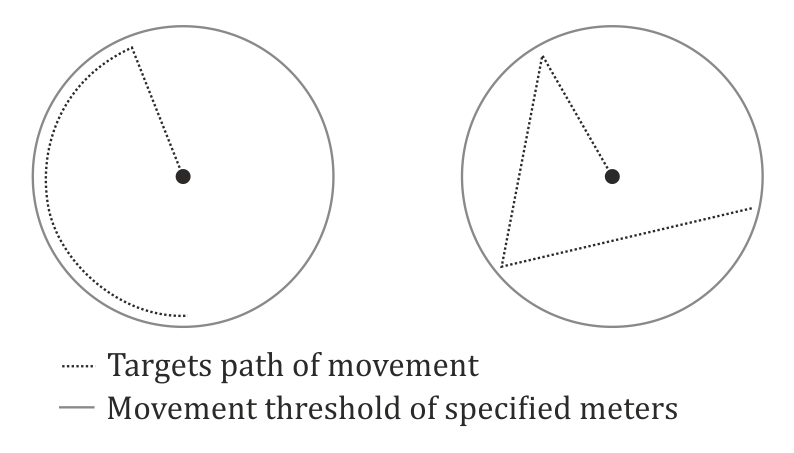
\includegraphics{UnevenMovement}
\label{unevenmovement}
\caption{Examples of how some kinds of movement can give trouble with the distance based algorithms}
\end{figure}

The left circle shows a target, which moves to the circumference of the movement threshold and then follow the circumference at the inside. It results in no location is sent to the server, due to the threshold is never crossed, and a lot of GPS fixes, due to the small distance to the circumference.

The right circle shows a situation, where the target moves in one direction and then change direction to backwards. If the target only moves around inside the threshold circle the server will not get any location updates.

These conditions has to be evaluated according to the use case, where it can be determined whether these scenarios will occur. In the case where a person walks or a car drives towards some locations it is unlikely, that these scenarios will occur.

\section{Conclusion}
It is possible to reduce both the number of GPS fixes and the number of connections to servers, and still track the target. However the use case must be taking into account, due the different limitations of the algorithms. Commonly they are best suited for targets, which primary move at a straight paths. But with these algorithms the battery consumption can be reduced and devices can use pervasive positioning for longer time.

\section{Appendix - Google Earth}
Full size images and data is found in code.zip in the folders experimentImages and experimentLogs.

\begin{figure}[ht]
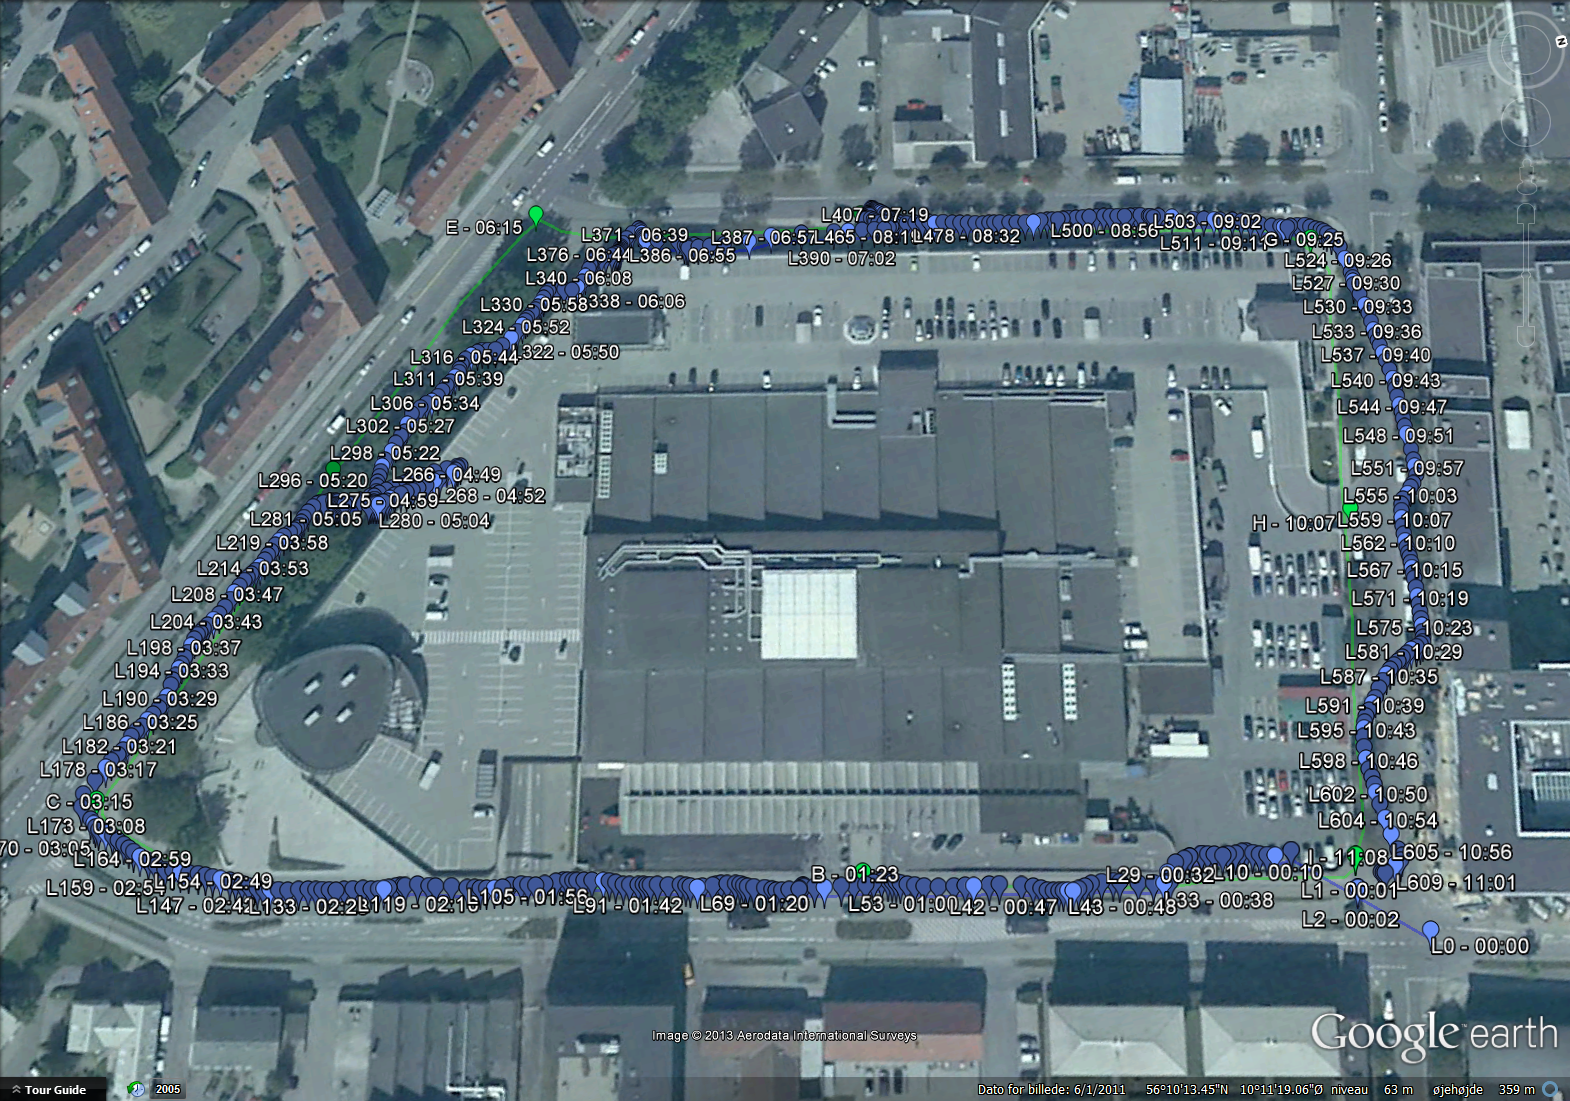
\includegraphics[scale=0.2]{figures/periodicRSAll}
\caption{Periodic readings with all locations shown. Green is ground truth, blue is the actual reading}
\end{figure}

\begin{figure}[ht]
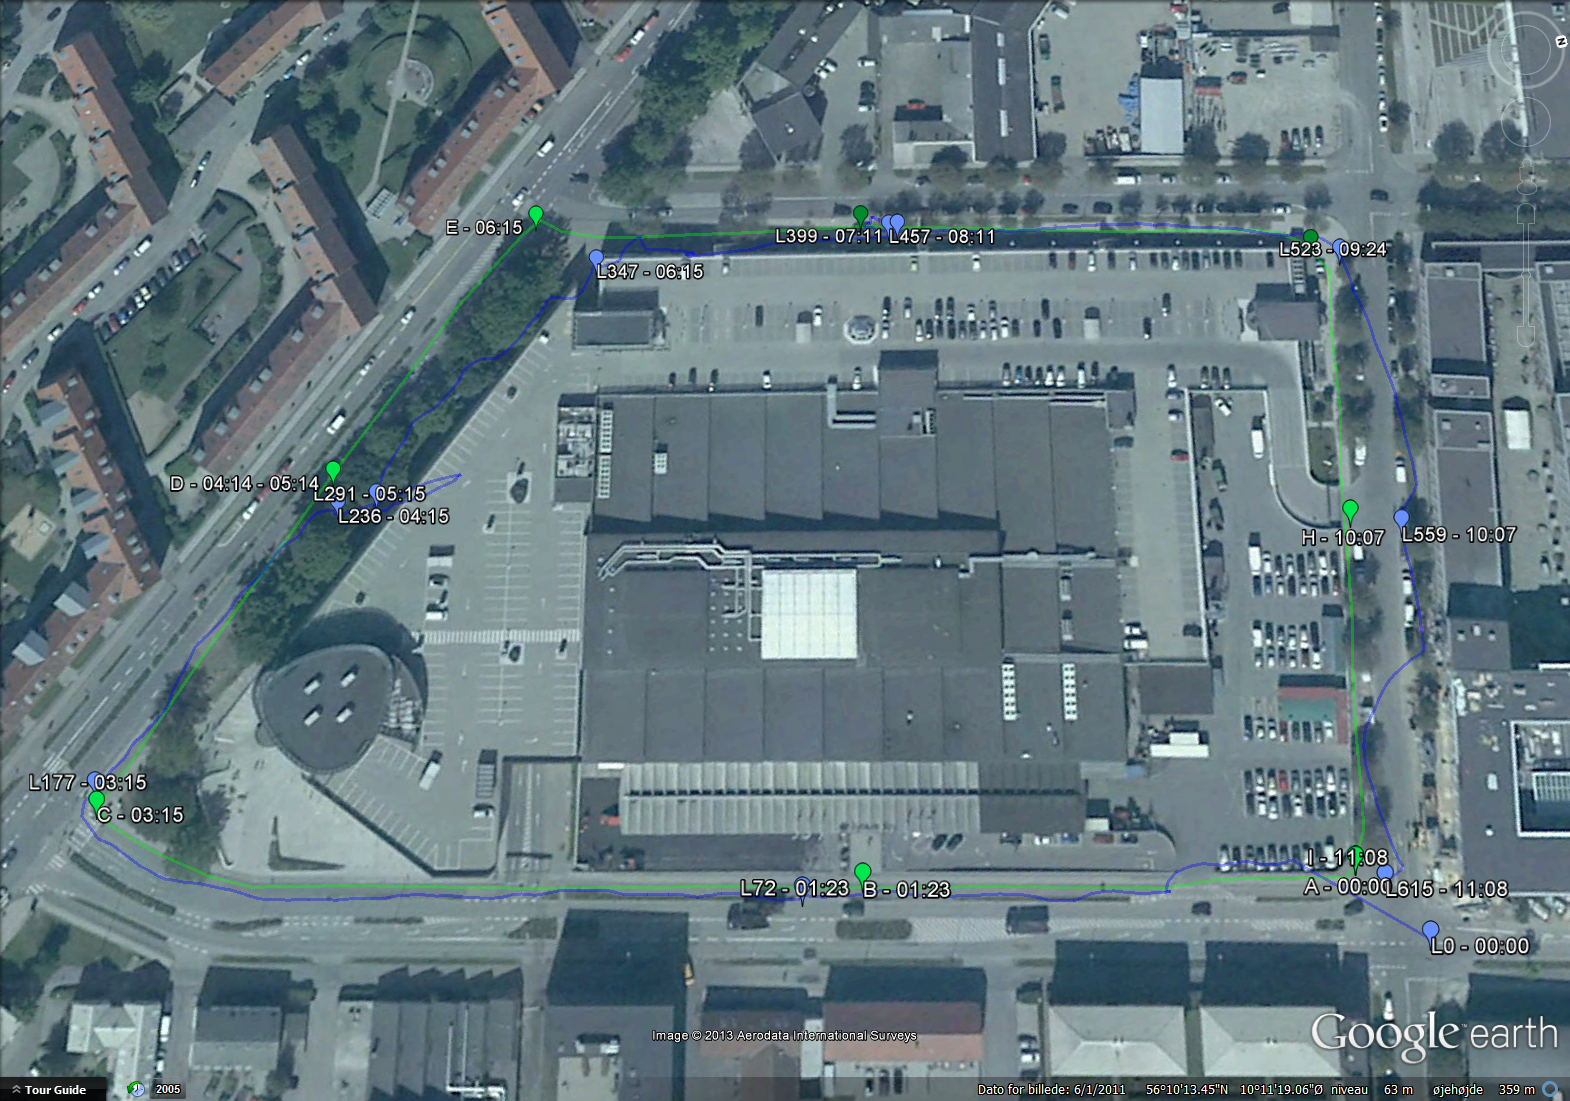
\includegraphics[scale=0.2]{figures/periodicRS}
\caption{Periodic readings filtered to show readings close to the ground truth. Green is ground truth, blue is the actual reading}
\end{figure}

\begin{figure}[ht]
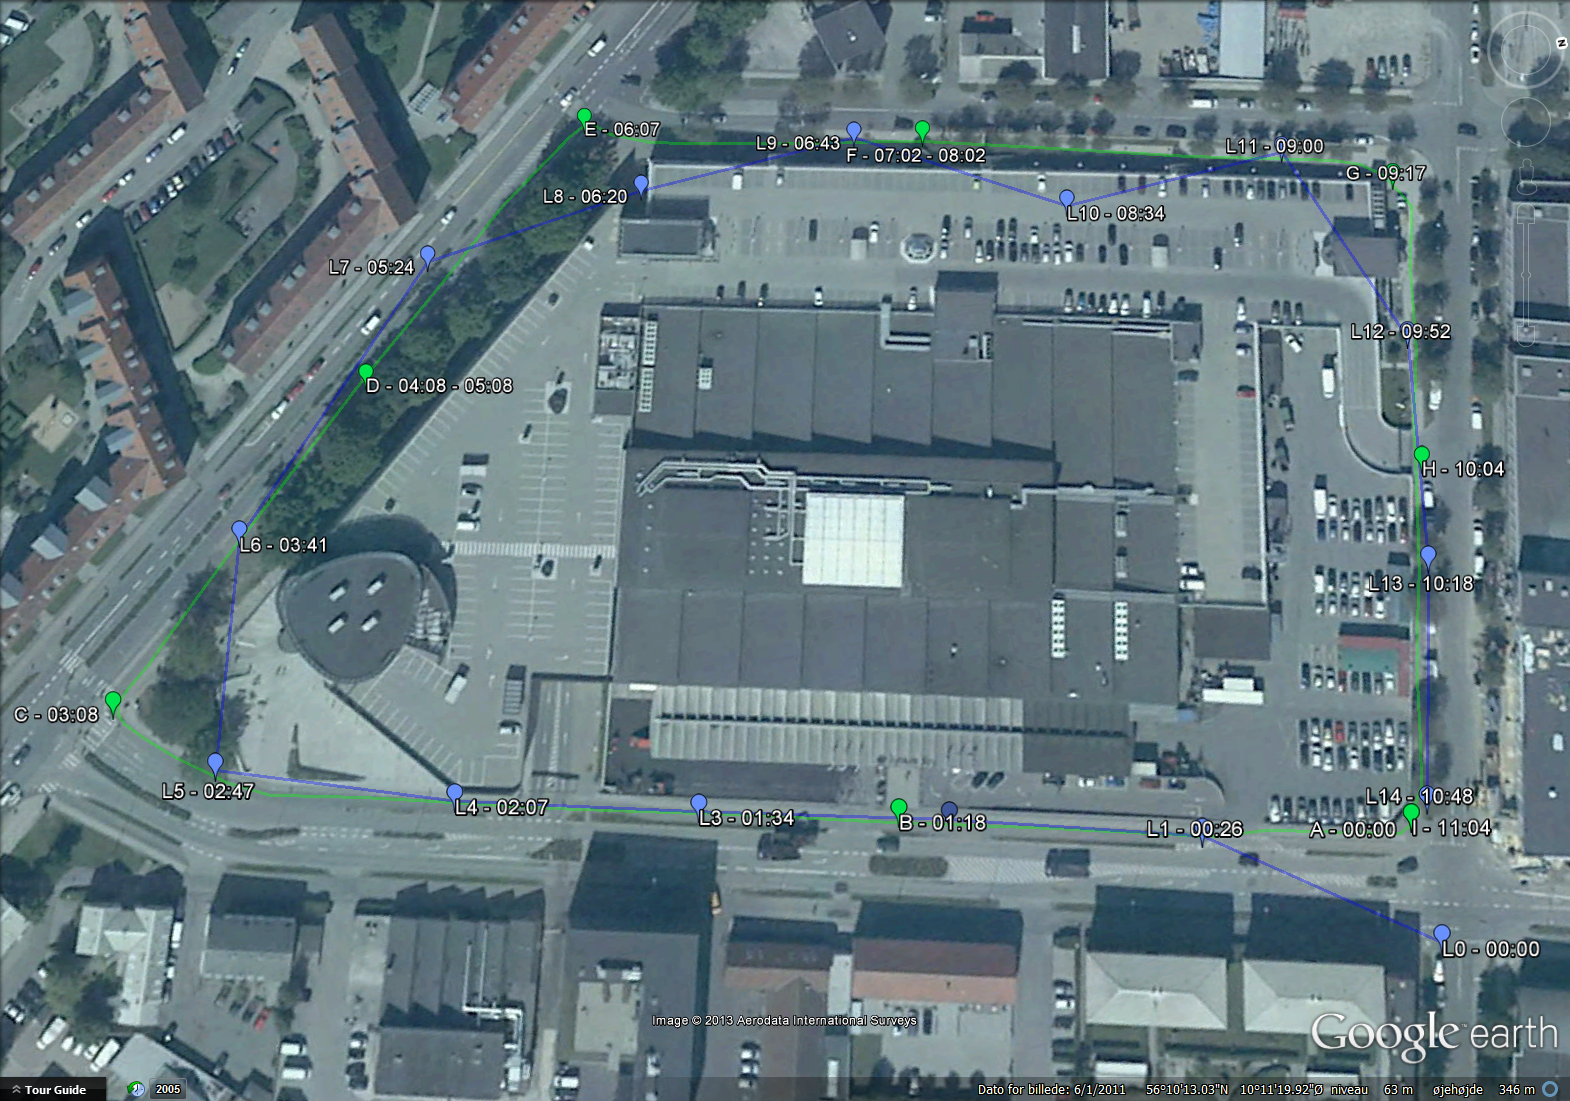
\includegraphics[scale=0.2]{figures/distanceBRS}
\caption{Distance based readings. Green is ground truth, blue is the actual reading}
\end{figure}

\begin{figure}[ht]
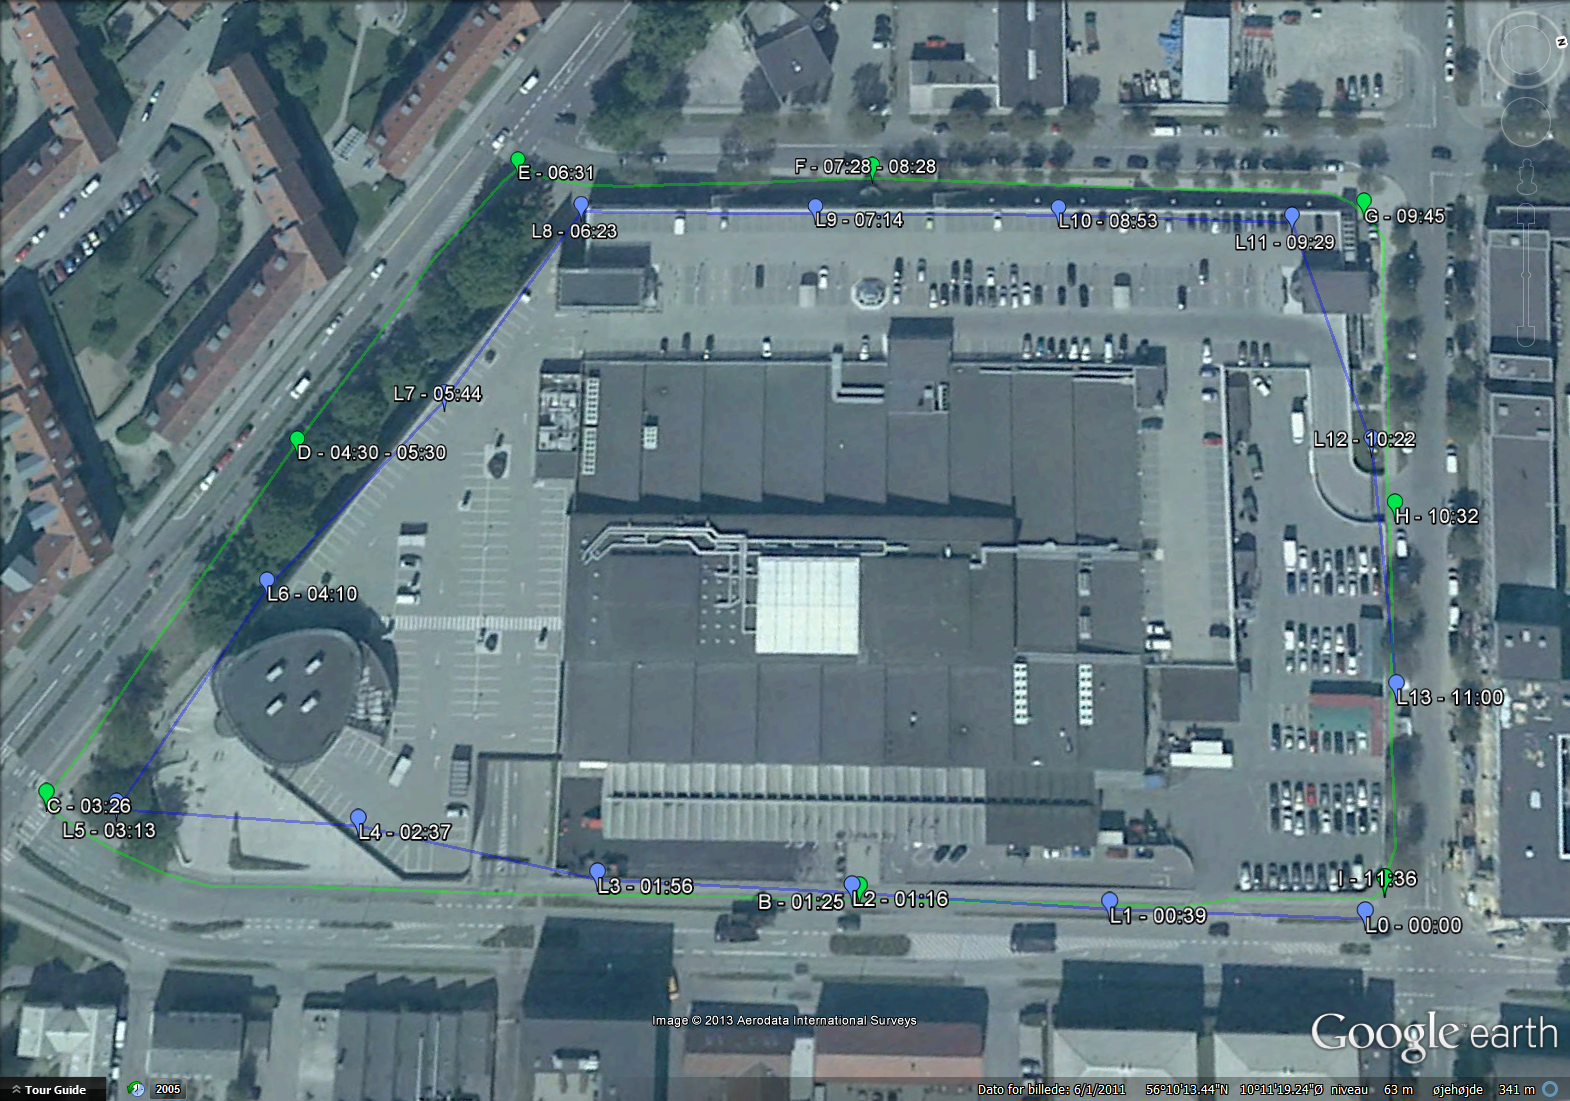
\includegraphics[scale=0.2]{figures/DBRSAccelerometer}
\caption{Distance based with accelerometer readings. Green is ground truth, blue is the actual reading}
\end{figure}

\begin{figure}[ht]
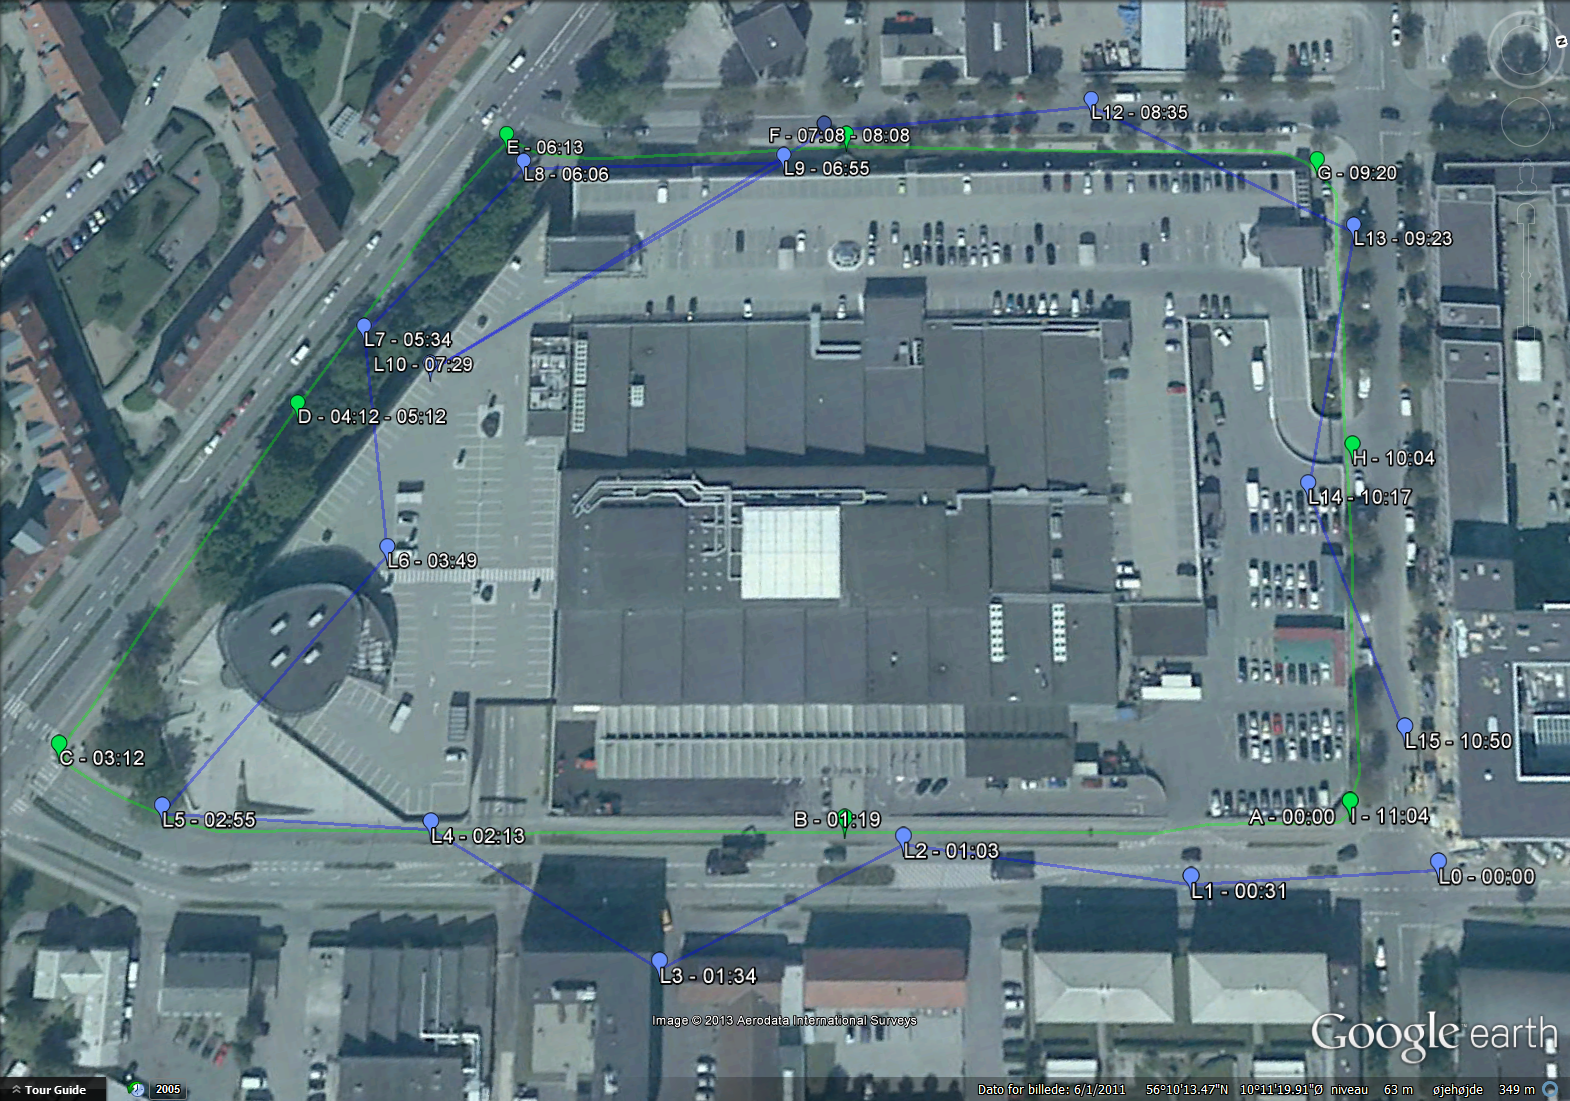
\includegraphics[scale=0.2]{figures/DBRSMaxSpeed}
\caption{Distance based with maximum speed readings. Green is ground truth, blue is the actual reading}
\end{figure}

\end{document}
